% Figure from MATH 591 notes, section 60 (added, not from lecture). Compile with the notes preamble.
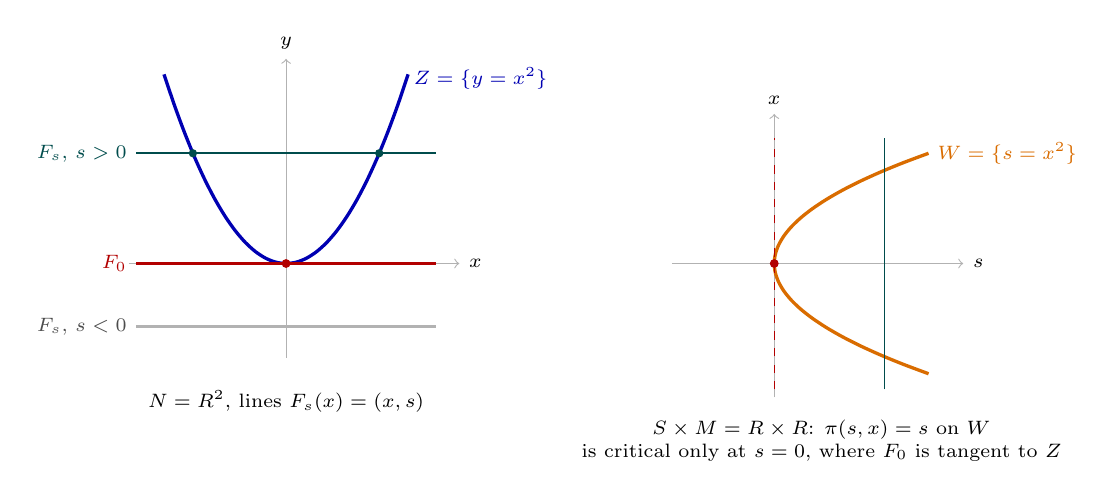
\begin{tikzpicture}[scale=1.0, font=\scriptsize]
% left: N = R^2, Z = parabola, F_s(x) = (x,s)
\begin{scope}
\draw[->, gray!60] (-2,0) -- (2.2,0) node[right, text=black] {$x$};
\draw[->, gray!60] (0,-1.2) -- (0,2.6) node[above, text=black] {$y$};
\draw[blue!70!black, very thick] plot[smooth, domain=-1.55:1.55] (\x,{\x*\x});
\node[blue!70!black, anchor=west] at (1.5,2.35) {$Z = \{y = x^2\}$};
\foreach \s/\c in {1.4/teal!60!black, 0/red!70!black, -0.8/gray!60} {\draw[\c, thick] (-1.9,\s) -- (1.9,\s);}
\node[teal!60!black, anchor=east] at (-1.9,1.4) {$F_s$, $s > 0$};
\node[red!70!black, anchor=east] at (-1.9,0) {$F_0$};
\node[gray!60!black, anchor=east] at (-1.9,-0.8) {$F_s$, $s < 0$};
\fill[teal!60!black] ({sqrt(1.4)},1.4) circle (1.5pt); \fill[teal!60!black] ({-sqrt(1.4)},1.4) circle (1.5pt);
\fill[red!70!black] (0,0) circle (1.6pt);
\node[align=center] at (0,-1.75) {$N = \mathbb{R}^2$, lines $F_s(x) = (x, s)$};
\end{scope}
% right: S x M with W = {s = x^2}
\begin{scope}[xshift=6.2cm]
\draw[->, gray!60] (-1.3,0) -- (2.4,0) node[right, text=black] {$s$};
\draw[->, gray!60] (0,-1.7) -- (0,1.9) node[above, text=black] {$x$};
\draw[orange!85!black, very thick] plot[smooth, domain=-1.4:1.4] ({\x*\x},\x);
\node[orange!85!black, anchor=west] at (1.95,1.4) {$W = \{s = x^2\}$};
\draw[red!70!black, dashed] (0,-1.6) -- (0,1.6);
\draw[teal!60!black] (1.4,-1.6) -- (1.4,1.6);
\fill[red!70!black] (0,0) circle (1.6pt);
\node[align=center] at (0.6,-2.25) {$S \times M = \mathbb{R} \times \mathbb{R}$: $\pi(s,x) = s$ on $W$\\ is critical only at $s = 0$, where $F_0$ is tangent to $Z$};
\end{scope}
\end{tikzpicture}
